
% \documentclass[aip,jcp,preprint,unsortedaddress,a4paper,onecolum]{revtex4-1}
\documentclass[]{tMPH2e}
% \documentclass[aps,pre,twocolumn]{revtex4-1}
% \documentclass[aps,jcp,groupedaddress,twocolumn,unsortedaddress]{revtex4}

% \usepackage[fleqn]{amsmath}
% \usepackage{amssymb,amsthm}
% \usepackage[dvips]{graphicx}
\usepackage{color}
% \usepackage{tabularx}
% \usepackage{algorithm}
% \usepackage{algorithmic}

\makeatletter
\makeatother


\newtheorem{thm}{Theorem}

\newcommand{\recheck}[1]{{\color{red} #1}}
\newcommand{\redc}[1]{{\color{red} #1}}
\newcommand{\bluec}[1]{{\color{blue} #1}}
\newcommand{\vect}[1]{\textbf{\textit{#1}}}
\newcommand{\dd}{\textsf{d}}
\newcommand{\inv}{\textrm{inv}}


\newcommand{\R}{{\mathbf R}}
\newcommand{\Q}{{\mathbf Q}}
\newcommand{\Z}{{\mathbf Z}}
\newcommand{\N}{{\mathbf N}}
\newcommand{\T}{{\mathbf T}}
\newcommand{\mh}{\mathcal H}
\newcommand{\eps}{\varepsilon}
\newcommand{\ml}{\mathcal L}
\newcommand{\mt}{\mathcal T}
\newcommand{\mo}{\mathcal O}
\newcommand{\mi}{\mathcal I}
\newcommand{\mc}{\mathcal C}
\newcommand{\proj}{\mathit\Pi}
\newcommand{\fwg}{{\mathcal A}}
\newcommand{\cA}{\mathcal A}
\newcommand{\cU}{\mathcal U}
\newcommand{\bwg}{{\mathcal B}}
\newcommand{\bsigma}{\boldsymbol\sigma}
\newcommand{\bE}{{\mathbf E}}
\newcommand{\bP}{{\mathbf P}}
\newcommand{\one}{{\mathbf 1}}
\newcommand{\zero}{{\mathbf 0}}

\newcommand{\wrt}{with respect to }


\begin{document}

\title{Linear response theory and optimal control for a molecular system under nonequilibrium conditions}

\author{Han Wang$^{a}$ and Carsten Hartmann$^{a}$ and Christof Sch\"utte$^{a,b}$$^{\ast}$\thanks{$^\ast$Corresponding author. Email: Christof.Schuette@fu-berlin.de}\\\vspace{6pt}$^{a}${\em Institute for Mathematics, Freie Universit\"at Berlin, Germany}\\$^{b}${\em Zuse Institute Berlin (ZIB), Germany}}
  

% \author{Han Wang}
% \author{Carsten Hartmann}
% \affiliation{Institute for Mathematics, Freie Universit\"at Berlin, Germany}
% \author{Christof Sch\"utte}
% \affiliation{Institute for Mathematics, Freie Universit\"at Berlin, Germany}
% \affiliation{Zuse Institute Berlin (ZIB), Germany}
% \affiliation{Institute for Mathematics, Freie Universit\"at Berlin, Germany}

\maketitle

\begin{abstract}
  In this paper, we propose a straightforward generalization of linear response theory on a finite time-horizon to systems in nonequilibrium that are subject to external forcing driving.  We briefly revisit the standard linear response result for equilibrium systems, where we consider Langevin dynamics as a special case, and then give an alternative derivation using a change-of-measure argument that does not rely on any stationarity or reversibility assumption. This procedure easily enables us to calculate the second order correction to the linear response formula (which may or may not be useful in practice). Furthermore, we outline how the novel nonequilibrium linear response formula can be used to compute optimal controls of molecular systems for cases in which one wants to steer the system to maximize a certain target expectation value. We illustrate our approach with simple numerical examples. 
\end{abstract}


\section{Introduction}

Standard molecular dynamics simulations are dealing with systems in thermal equilibrium; in this case they are tuned to the canonial or Boltzmann distribution in the sense that either (1) if one starts from this distribution it remains invariant under the dynamics or (2) if one generates a very long trajectory it samples state space with respect this distribution, that is, every possible state of the molecular system under consideration is visited according to the probability given by it.  Obviously, this allows to compute equilibrium expectation values with respect to the  canonical distribution simply be computing long trajectories. 

Often, however, one is interested in knowing about the response of the molecular system to perturbation out of equilibrium. The standard linear response formula allows to answer this question, at least partially. In the standard setting it gives us the first order of the change to an equilibrium expectation value as resulting from the nonequilibrium perturbation. Here, first order means first order in the size of the perturbation. This linear response formula has a long history of extensions and generalizations; see, e.g., \cite{marconi2008,ruelle2009} and the references therein. In some sense it has become one of the cornerstones of modern statistical physics since it can be related to the fluctuation dissipation theorem (FDT) which roughly states that for appropriate systems in statistical equilibrium, the average response to small external perturbations can be calculated through the knowledge of suitable correlation functions of the unperturbed statistical system. Linear response formulae on the infinite time-horizon have been shown to hold under rather mild assumptions and for nonequilibrium systems with a unique invariant measure \cite{hairer2008}. 

There is an increasing number of articles in the literature that report on applications of molecular dynamics to nonequilibrium settings. There are many generalization to so-called nonequilibrium steady states based on the generality of the FDT \cite{Seifert}, but despite its wide use, we are not aware of a linear response formula, even for nonequilibrium (i.e.~irreversible) systems, that does not rely on any kind of stationarity assumption. We will provide such a formula for the case that the underlying dynamics can be described by Langevin dynamics that may not have an invariant measure. Furthermore, we will provide a formula for the second order response of a nonequilibrium Langevin system subject to a small perturbation.

Instead of applying this theory to a molecular system we will go one step further. We will outline how the novel nonequilibrium linear response formula can be used to compute the optimal control of molecular systems. In optimal control one seeks the optimal way to perturb a molecular system such that a certain target expectation value (e.g. population of certain states) is maximized under constraints on the energy of the control. In general the control drives the molecular system under control out of equilibrium. Thus, the nonequilibrium linear response formula can be used to find the optimal correction of the present control regarding the expectation value of interest. 

The outline of the article is as follows: First, we will review the derivation of finite time-horizon linear response formulae for general diffusion processes and diffusions of Langevin type. Next, we will show how to derive first and second order response formulas for genuine nonequilibrium systems and how to apply these formula to the computation of optimal controls. Finally, we will validate the nonequilibrium linear response formula and its use for optimal control for simple test cases. This numerical experiments will also outline that the use of the linear response formula is imperative for numerical efficiency and allows to extend the applicability of linear response theory to stronger perturbations. 


 

\section{Linear response}


In this section, we first want to give a simple and formal derivation of the linear response for equilibrium and nonequilibrium systems. To this end we consider a general It\^o stochastic differential equation of the form
\begin{equation}\label{sde}
dX_{t} = (b(X_{t},t) + \eps v_{t})dt +a(X_{t})dB_{t}\,,\quad t\ge 0\,,
\end{equation}
where $X_{t}\in\R^{d}$, $b(\cdot,\cdot)$ is a smooth time-dependent vector field, $a(\cdot)$ a smooth field of $d\times n$ matrices and $B_{t}$ is standard Brownian motion in $\R^{n}$. Here $v_{t}\in\R^{d}$ is any given driving force applied to the system, typically an affine function of the form $v_{t}=B(X_{t})u(t)$, with $B(\cdot)\in\R^{d\times k}$ and a bounded measurable function $u\colon[0,\infty)\to\R^{k}$ such that (\ref{sde}) has a strong solution for all $t> 0$ whenever $\eps>0$ is sufficiently small. When (\ref{sde}) without the perturbation $\eps v$ is considered, we write
\begin{equation}\label{sdewo}
dx_{t} = b(x_{t},t)dt +a(x_{t})dB_{t}\,,\quad t\ge 0\,. 
\end{equation}


  




\subsection{Small perturbations from equilibrium: Langevin dynamics}

We consider the equilibrium and nonequilibrium case separately and start with the equilibrium case (see, e.g., \cite{kubo1957,tuckerman2010statistical}). To begin with, we assume that the perturbation-free part of the infinitesimal generator
\[
\fwg^{\eps} = \fwg_{0} + \eps\fwg_{1}\,, 
\]
of (\ref{sde}) with 
\[
\fwg_{0} = \frac{1}{2}aa^{T}\colon\nabla^{2} + b\cdot\nabla\,,\quad \fwg_{1}=v\cdot\nabla 
\]
has an isolated eigenvalue 0 corresponding to the unique invariant measure $d\mu_{\infty}=\rho_{\infty}dx$. We denote by $\cA_{0}^{*}$ and $\cA_{1}^{*}$ the formal adjoints in $L^{2}$, e.g., $\cA_{1}^{*}\phi=-\nabla(v \phi)$.  


Now let $f\colon\R^{2n}\to\R$ be any integrable function and let $\rho^{\eps}=\rho^{\eps}(x,t)$ denote the probability density of $X_t$, at time $t>0$, assuming that $X_{0}=x$ was distributed according to $\rho^{\eps}(x,0)=\rho_{\infty}(x)$. We define the expectation \wrt $\rho^{\eps}$ as 
\[
\bE_{\rho^{\eps}}[f] = \int_{\R^{2n}} f(x) \rho^{\eps}(x,t) \,dx\,.
\] 
A classical result, that is usually derived using a formal expansion of the solution to the Fokker-Planck equation in powers of $\eps$ using the ansatz 
\[
\rho^{\eps}(x,t)=\rho_{0}(x,t) + \eps\rho_{1}(x,t) + \ldots\] 
with 
\[\rho^{\eps}(x,0)=\rho_{\infty}\,,\textrm{ i.e. }\; \rho_{0}(x,0)=\rho_{\infty}\textrm{  and  } \rho_{i}(x,0)=0\textrm{ for $i>0$},
\] 
then states that (see, e.g., \cite{tuckerman2010statistical,hartmann2010})
\begin{equation}\label{lr}
\lim_{\eps\to 0}\frac{\bE_{\rho^{\eps}}[f] - \bE_{\rho^{0}}[f]}{\eps} =\int_{\R^{2n}}f(x)\left(\int_{0}^{t}e^{\cA_{0}^{*}(t-s)}\cA_{1}^{*}(s)\rho_{\infty}(x)\,ds\right)dx\,.
\end{equation}


\subsubsection*{Green-Kubo relations} 

Specifically, we are interested in the case that (\ref{sde}) has the form of a second-order Langevin equation, in which case $d=2n$ and 
\begin{equation}\label{eqn:langevin-1}
b(x,t) = (J-R)\nabla H(x)\,,\quad a = \sqrt{2\beta^{-1}}R^{1/2}\,,
\end{equation}
with $J=-J^{T}$ the canonical $2n\times 2n$ symplectic matrix,
\[
J = \left ( \begin{array}{cc} 
0 & I_{n\times n} \\ -I_{n\times n} &0
\end{array}\right),
\]
$R=R^{T}\ge 0$ the positive semidefinite $2n\times 2n$ friction matrix 
\[
R = \left ( \begin{array}{cc}
0 & 0 \\ 0 & \gamma
\end{array}\right),
\]
for $\gamma\in\R^{n\times n}$ symmetric positive definite, and 
\[
H\colon\R^{2n}\to\R\,,\quad H(x) = \frac{1}{2}|x_{2}|^{2} + V(x_{1})
\] 
the Hamiltonian of the system. We assume that the potential $V$ is bounded from below. Then, under some mild growth conditions on $V$ for $|x_{1}|\to\infty$ (see, e.g., \cite{mattingly2002}), the unperturbed dynamics has a unique invariant measure with density 
\[
\rho_{\infty}(x) = \frac{1}{Z}\exp(-\beta H(x))\,,\quad  Z=\int_{\R^{2n}}  \exp(-\beta H(x))\,dx\,.
\] 
In this case, the linear response result (\ref{lr}) can be recast in form of the better known Green-Kubo formula \cite{risken1996}. Assuming that the forcing is of the form $v_{t}=Bu(t)$ with $u\colon[0,\infty)\to\R^{n}$ and $B\in\R^{2n\times n}$ being any given time-dependent function, the above expression can be recast as 
\begin{equation}\label{GreenKubo}
\lim_{\eps\to 0}\frac{\bE_{\rho^{\eps}}[f] - \bE_{\rho^{0}}[f]}{\eps} = \beta\int_{0}^{t}F(t-s)u(s)\,ds
\end{equation}
where 
\[
F(t) = - \int_{\R^{2n}}\bE_{x}[f(x_{t})] B^{T}\nabla H(x)\rho_{\infty}(x)\,dx
\]
is the response function and the expectation under the integral is taken over all realization of the equilibrium process (\ref{sdewo}) starting from $x_{0}=x$. In other words: 
\[
\bE_{\rho^{\eps}}[f] \approx \bE_{\rho_{\infty}}[f] + \eps\beta\int_{0}^{t}F(t-s)u(s)\,ds\,,
\]
where we have used the fact that $\rho^{0}(x,t)\to \rho_{\infty}(x)$ uniformly on $\R^{2n}\times[0,\infty)$. 
 
\paragraph*{Remark.}
It is possible to extend the above framework to the case of observables that are functionals of the path, i.e.~to functions the form 
\[
\varphi^{\eps}(x,t) = \bE_{x}\left[\int_{0}^{t}f(X_{s})ds\right]\,,
\]
where the expectation is over all realizations of the \emph{nonequilibrium} process $X_{t}$ with initial condition $X_{0}=x$. In this case a linear response result can be obtained by expanding the solution of the Kolmogorov backward equation
\[
\frac{\partial\varphi^{\eps}}{\partial t} = \cA^{\eps}\varphi^{\eps} - f\,,\quad \varphi^{\eps}(x,0) = 0\,, 
\]
rather than the Fokker-Planck equation, where the equivalence between the solution of the backward equation and the conditional expectation of the path functional follows from the Feynman-Kac formula \cite[Thm.~1.3.17]{pham2009}. 





%%%%%%%%%%%%%%%%%%%%%%%%%%%%%%%%%%%%%%%%%%%%%%%%%%%%%%%%%%%%%%%%%%%%%%%%%%%%%%%%%%%%%%%%%%%%%%%%%%%%%%%%%
%%%%%%%%%%%%%%%%%%%%%%%%%%%%%%%%%%%%%%%%%%%%%%%%%%%%%%%%%%%%%%%%%%%%%%%%%%%%%%%%%%%%%%%%%%%%%%%%%%%%%%%%%

\subsection{Nonequilibrium response theory: controlled Langevin dynamics}

The derivation of the classical response result heavily relies on the fact that the unperturbed system has a unique equilibrium distribution, which requires that the generator of the process has certain spectral properties; cf.~\cite{hairer2008,stoltz2012}. Moreover the usual perturbation argument does not provide a framework, under which the second and even higher order responses can easily be derived. Here we propose an alternative derivation of the linear response result, that is based on a change of drift in the corresponding SDE and which allows for an easy generalization of the above linear response result to nonequilibrium systems.

\subsubsection*{Girsanov transformation}
We will briefly review the idea of the change of drift via Girsanov transformations; for details we refer to the textbook \cite{oksendal2003stochastic}. To this end, let $x_{t}=x_{t}(\omega)$ and $X_{t}=X_{t}(\omega)$ be the solutions of our generic stochastic differential equations
\begin{subequations}\label{sde2}
\begin{align}
dx_{t} & = b(x_{t},t)dt + a(x_{t})dB_{t}\,,\quad 0\le t\le T  \label{sde2-1}\\
dX_{t} & = (b(X_{t},t) + \eps v_{t})dt +a(X_{t})dB_{t}\,,\quad 0\le t\le T \label{sde2-2}
\end{align}
\end{subequations}
for $T<\infty$ and deterministic initial conditions
\[
x_{0}(\omega) = X_{0}(\omega) = x\quad\textrm{(almost surely)}\,.
\]
Suppose that there exists an auxiliary stochastic process $\xi_{t}\in\R^{m}$ such that 
\begin{equation}\label{xi}
a(X_{t})\xi_{t} = v_{t}\,.
\end{equation}
The auxiliary variable $\xi$ will be called \emph{control variable}. We define  
\[
W_{t} = \eps\int_{0}^{t}\xi_{s}\,ds + B_{t}\,,\quad 0\le t\le T\,,
\]
which allows us to rewrite (\ref{sde2-2}) as
\begin{equation}\label{sde2-3}
dX_{t} = b(X_{t},t)dt +a(X_{t})dW_{t} 
\end{equation}
It follows from the Girsanov theorem \cite[Thm.~8.6.8]{oksendal2003stochastic}, sometimes also called \emph{Cameron-Martin-Girsanov theorem} \cite{stroock2006}, that $W_{t}$ is again a Brownian motion under a new probability measure that has a density \wrt the Gaussian probability measure that is generated by the Brownian motion $B_{t}$. Specifically, let $\nu$ denote the law of the Brownian motion $B_{t}$ and define a new probability measure $\mu$ on the space of continuous trajectories by 
\[
d\mu=M_{T}d\nu
\]
with 
\begin{equation}\label{likelihood}
M_{t} = \exp\left(-\eps\int_{0}^{t}\xi_{s}\cdot dB_{s} - \frac{\eps^{2}}{2}\int_{0}^{t}|\xi_{s}|^{2}ds\right)\,,\quad 0\le t\le T\,.
\end{equation}
Technical details aside, the Girsanov theorem implies that $W_{t}$  for any functional 
\[
\varphi(\omega)=\int_{0}^{T}f((X_{s}(\omega))\,ds + g(X_{T}(\omega))
\] 
that is integrable \wrt $\nu$, we have the identity\footnote{One of the omitted technical details is Novikov's condition \cite[pp.~162]{oksendal2003stochastic} that guarantees that $(M_{t})_{0\le t\le T}$ is a Martingale, which by $\bE_{\mu}[1]=\bE_{\nu}[M_{T}]=1$ implies normalizability of the new probability measure $\mu$.}
\[
\bE_{\nu}[\varphi] := \int_{\Omega} \varphi(\omega)\, d\nu(\omega) = \int_{\Omega} \varphi(\omega) M_{T}^{-1}(\omega)\,d\mu(\omega) =: \bE_{\mu}[M^{-1}_{T}\varphi]\,.
\]
where 
\[
M_{T}^{-1} = \exp\left(\eps\int_{0}^{T}\xi_{s}\cdot dW_{s} - \frac{\eps^{2}}{2}\int_{0}^{T}|\xi_{s}|^{2}ds\right)
\]
is the density of $\nu$ relative to $\mu$. Note that the expectation on the right hand side corresponds to the unperturbed dynamics, because $W_{t}$ is a standard Brownian motion under $\mu$, and the expectation is over all realizations of (\ref{sde2-3}) starting from either any given initial condition $X_{0}=x$ or an arbitrary initial distribution. On the other hand, $X_{t}$ under $\nu$ corresponds to the perturbed dynamics, which should become clear upon comparing equations (\ref{sde2-2}) and (\ref{sde2-3}). 


\paragraph*{Remark.} 

A quick-and-dirty derivation of the above change-of-measure formula can be easily obtained, if the noise covariance $a(\cdot)a(\cdot)^{T}$ has full rank with bounded inverse. Then, using Euler's method for (\ref{sde2}), it follows that (\ref{likelihood}) is basically the likelihood ratio between the time-discrete path densities of (\ref{sde2-2}) and (\ref{sde2-1}).  Another route to the same result is by using the Onsager-Machlup functional \cite{Pinski1} for $(X_t)_{0\le t\le T}$ and $(x_t)_{0\le t\le T}$; then $M_{T}$ is found as the likelihood ratio of the two densities. 






\subsubsection*{An alternative linear response formula}

Linearization of $M_{T}^{-1}$ about $\eps=0$, assuming that the control has bounded variance, yields the alternative linear response formula 
\begin{equation}\label{lr-alt}
\lim_{\eps\to 0}\frac{\bE_{\rho_{x}^{\eps}}[\varphi] + \bE_{\rho_{x}^{0}}[\varphi]}{\eps} = \bE_{\rho_{x}^{0}}\left[\varphi \int_{0}^{T}\xi_{s}\cdot dB_{s} \right]\,,
\end{equation}
where, in accordance with the previous linear response formula, $\rho_{x}^{\eps}$ and $\rho_{x}^{0}$ denote the path probability distributions of perturbed and unperturbed processes (\ref{sde2-2}) and (\ref{sde2-1}) with deterministic initial condition. On the right hand side of the last equation $\varphi$ is understood as a functional of $(x_{t})_{0\le t\le T}$, the solution to (\ref{sde2-1}) with initial condition $x_{0}=x$, and $\xi_{t}$ is the solution to $a(x_{t})\xi_{t}=v_{t}$. By averaging the the initial values $x$ on both sides of (\ref{lr-alt}) over any given initial distribution, one obtains an analogous formula for distributed initial conditions.  

Note that $\varphi$ and $B_{t}$ are not independent, hence the product of $\varphi$ and the integral over the Brownian motion does not average to zero in general. 


\paragraph*{Remark.} 
By formally expanding $M^{-1}_T$ up to second order we get an analogous second order response formula: 
\begin{equation}\label{2nd}
\begin{aligned}
\bE_{\rho_{x}^{\eps}}[f] & \approx \bE_{\rho_{x}^{0}}[\varphi]  + \eps \bE_{\rho_{x}^{0}}\left[\varphi\int_{0}^{T}\xi_{s}\cdot dB_{s} \right]\\  
& + \frac{\eps^{2}}{2} \bE_{\rho_{x}^{0}}\left[\varphi\left\{\left(\int_{0}^{T}\xi_{s}\cdot dW_{s}\right)^2 -\int_0^T |\xi_s|^2\,ds\right\} \right].
\end{aligned}
\end{equation}


 
 

\subsubsection*{Nonequilibrium Langevin Dynamics}

We now link our previous considerations with the previous case and consider a nonequilibrium Langevin equation. Specifically, we add a non-gradient perturbation to the drift (\ref{eqn:langevin-1}) of the previous Langevin equation, i.e., we set 
\begin{equation}\label{eqn:langevin-1b}
b(x,t) = (J-R)\nabla H(x) +  B(x) u(t)\,,\quad a(x) = \sqrt{2\beta^{-1}}R^{1/2}
\end{equation}
with the definitions of $J,R$ and $H$ unchanged, $u\in\R^{n}$ being some control variable, and $B(\cdot)\in\R^{2n\times n}$ given by 
\[
B(x) = \left( \begin{array}{c}
0 \\ D(x) \end{array}\right)
\]
The matrix $D(\cdot)\in\R^{n\times n}$ must be chosen such that $B$ satisfies the Fredholm alternative $\mathrm{range}(B(\cdot))\perp \mathrm{ker}((a(\cdot))^{T})$, where $\mathrm{ker}(a^T)$ denotes the kernel of $a^T$. 

We are interested in the dynamics under a small perturbation $\delta u$ of the control $u$, Specifically, we assume that $v$ in (\ref{sde2}) is of the form 
\begin{equation}\label{eqn:langevin-1c}
v_{t} = B(X_{t})\delta u(t)
\end{equation}
so that equation (\ref{xi}) that determines the change of measure in terms of the auxiliary control variable $\xi$ (and thus the linear response) reads 
\[
\sqrt{2\beta^{-1}}R^{1/2} \xi_{t} = D(X_{t})\,\delta u_{t}\,.
\]
Hence the equation for $\xi_{t}$ is solvable if and only if $\mathrm{range}(D(\cdot))\perp \mathrm{ker}(R^{1/2})$, which, since $R$ has full rank, means that $D(\cdot)$ must be invertible almost everywhere.

To be more explicit, the equation we are considering has the form
\begin{equation}\label{eqn:langevin-1d}
dX_t =  (J-R)\nabla H(X_{t})dt + B(X_t)(u(t)+\eps \delta u(t))dt+a\, dB_t\,.
\end{equation}
In this case the linear response formula (\ref{lr-alt})  becomes
\begin{equation}\label{lr-alt2}
\lim_{\eps\to 0}\frac{\bE_{\rho_{x}^{\eps}}[\varphi] - \bE_{\rho_{x}^{0}}[\varphi]}{\eps} =  \bE_{\rho_{x}^{0}}\left[\varphi\int_{0}^{T}(\sigma^{-1}D(x_{s})\,\delta u_{s})\cdot dB_{s} \right]\,
\end{equation}
with the shorthands $\sigma=\sqrt{2\beta^{-1}}R^{1/2}$ and 
\[
\varphi = \int_{0}^{T}f(x_{s})ds+g(x_{T})\,.
\]
In other words: 
\begin{equation}\label{eqn:neq-response}
\bE_{\rho_{x}^{\eps}}[\varphi] \approx \bE_{\rho_{x}^0}[\varphi] + \eps\bE_{\rho_{x}^0}\left[\varphi\int_{0}^{T}(\sigma^{-1}D(x_{s})\,\delta u_{s})\cdot dB_{s} \right]\,.
\end{equation}
Here, as before, the expectation on the right hand side of the linear response formula is over all realizations of (\ref{eqn:langevin-1d}) for $\eps=0$ starting at $x$; see also the remark below on the choice of initial conditions. 

\subsubsection*{Numerical realization}

As one can easily get lost in the various transformations and changes of measure, involving $\nu$, $\mu$, $\rho_{x}^{\eps}$, $\rho^{0}_{x}$ etc. it may be helpful to understand how the linear response formulas (\ref{lr-alt}) or (\ref{lr-alt2}) can be realized algorithmically. To this end, let $(x_0,\,x_{1},\,x_{2},\,x_{3},\ldots)$ with $x_{k}$ be the numerical realization of (\ref{sde2-1}). Let us further suppose that the initial value $x_{0}=x$ is fixed. The simplest possible numerical discretization would be the Euler scheme 
\[
x_{n+1} = x_{n} + \Delta t\, b(x_{n},t_{n}) + \sqrt{\Delta t}\,a(x_{n})\eta_{n+1}\,,\quad x_{0}=x\,, 
\]
with time step $\Delta t=t_{k+1}-t_{k}$ and $\eta_{k}$ i.i.d.~Gaussian random variables with mean 0 and unit covariance. (For a Langevin equation such as (\ref{eqn:langevin-1d}) the Euler scheme is not recommended, but the basic idea stays the same.) Now a simple unbiased estimator of the linear response---i.e. the right hand side in (\ref{lr-alt})---would be 
\begin{equation}\label{lr-est}
\hat{R} = \frac{1}{M}\sum_{i=1}^{M}\left\{f(\{x_{k}(\omega_{i})\}_{0\le k\le N})\sum_{j=0}^{N-1}\hat{\xi}_{i}(\omega_{i})\cdot \eta_{j+1}(\omega_{i})\right\}
\end{equation}
with $N=\lfloor T/\Delta t\rfloor$ and $x_{k}(\omega_{i})$ denoting the $i$-th realization of $x_{k}$, that is generated by the $i$-th realization $(\eta_{1}(\omega_{i}),\ldots,\eta_{k}(\omega_{i}))$ of the Gaussian noise sequence $(\eta_{k})_{k\in\N}$. The time-discrete control variable is given by  
\[
a(x_{k})\hat{\xi}_{k} = v_{t_{k}}
\]
for any given perturbation $v\colon[0,T]\to\R^{m}$. 


\paragraph*{Remarks.} Some comments on the above result are in order:
\begin{itemize}

\item[(i)] The rightmost term in \eqref{eqn:neq-response} is the linear 
  response to the reference nonequilibrium process (driven by $u_t$ with $\eps=0$).  From (\ref{2nd}) we can also get the second order response term. The latter is bounded if the controls have bounded second moment, which is a typical requirement in optimal control applications. Higher order moments need not exist. 

\item[(ii)] In the above derivation, we have tacitly assumed that the reference and the perturbed nonequilibrium processes start from the same initial value or
  have the same initial distribution. For fixed initial values (i.e.~points) this assumption cannot be relaxed (because otherwise $d\nu/d\mu$ does not exist). For distributed initial values, however, there is no problem for the unperturbed and perturbed dynamics to have different initial distribution as long as both distributions are strictly positive almost everywhere. In this case one can apply a similar reweighing approach between the initial distribution as we used it for the trajectory ensemble.  

\item[(iii)] If one wants to calculate the same expectation value for a family of nonequilibrium perturbations $\delta u_t$ then 
one does not need to repeat the calculations of \eqref{eqn:neq-response} for every member of the family. 
  If it is possible to
  express different $\delta u_t$ in the same basis, then the responses must only be
  calculated for the single basis functions. Then with a linear combination of the responses on basis functions, one can derive
  the responses for the whole family. This feature will be used below when discussing optimal control as an application of the linear response formula. 
  

\end{itemize}




%%%%%%%%%%%%%%%%%%%%%%%%%%%%%%%%%%%%%%%%%%%%%%%%%%%%%%%%%%%%%%%%%%%%%%%%%%%%%%%%%%%%%%%%%%%%%%%%%%%%%%%%%
%%%%%%%%%%%%%%%%%%%%%%%%%%%%%%%%%%%%%%%%%%%%%%%%%%%%%%%%%%%%%%%%%%%%%%%%%%%%%%%%%%%%%%%%%%%%%%%%%%%%%%%%%

\section{Application of the nonequilibrium response formula: optimal control}

The nonequilibrium linear response formula can be used for solving certain optimal control problems. To this end, let us remain in the setting of equations (\ref{eqn:langevin-1d})--(\ref{eqn:neq-response}) and assume that we are interested choosing the nonequilibrium forcing $u$, such that the expected value $\bE[f]$ of some utility function 
\[
f(u) = \int_{0}^{T}\left\{\ell (q_{s}) - \frac{1}{2}|u_{s}|^{2}\right\}\,dt + L(q_{T}) 
\]
is maximized where $q_{t}$ is the solution to the controlled Langevin equation (\ref{eqn:langevin-1d}) for $\eps=0$; the functions $\ell$ and $L$ are the running cost and the terminal cost, which are assumed to be continuous and bounded from above; without loss of generality, $\ell$ and $L$ are assumed to depend only on the positions. The quadratic term is a penalization that makes sure that the controls do not go through the roof \cite{schuette2012,hartmann2012}. Let us moreover assume that the controls are open-loop (i.e. without feedback) and can be represented by 
\[
u_{t} = \sum_{k=1}^K a_k \Phi_k(t)\,,\quad a_{k}\in \R\,,
\]
with suitably chosen time dependent, bounded and Lipschitz continuous vector fields $\Phi_k\colon[0,T]\to\R^{n}$, $k=1,\ldots,K$. %In principle we could even go for closed-loop (i.e.~feedback) controls by making $\Phi_{k}$ state dependent. 
We want to solve the optimal control problem
\begin{equation}\label{ocp1}
\begin{aligned}
 \max_{u\in\cU} \,& I(u)\quad \textrm{s.t.}\\
dq_t & =  \nabla_p H(q_t,p_t)dt\\
dp_t & =  -\nabla_q H(q_t,p_t)dt - \gamma \nabla_p H(q_t,p_t)dt + D(q_t)u_{t} dt+\sigma dB_t\,.
\end{aligned}
\end{equation}
where 
\begin{equation}\label{ocp2}
I(u) = \bE_{\rho^0}\left[\int_{0}^{T}\left\{\ell (q_{s}) - \frac{1}{2}|u_{s}|^{2}\right\}\,dt + L(q_{T}) \right]
\end{equation}
and $\cU$, the space of admissible controls, consists of all bounded controls 
\begin{equation}\label{admissible}
u_{t} = \sum_{k=1}^K a_k \Phi_k(t)\,,\quad a_{k}\in \R\,,
\end{equation}


\subsubsection*{Gradient method from linear response}

In principle optimal control problems such as (\ref{ocp1})--(\ref{ocp2}) can be solved by dynamic programming, i,e., by solving the corresponding Hamilton-Jacobi-Bellman PDE \cite{fleming2006}. Expect for very simple, essentially one-dimensional systems, solving Hamilton-Jacobi-Bellman equations is not an easy task, so we pursue a different strategy here. The idea is to use that we have restricted our space of admissible controls to functions of the form (\ref{admissible}) with given basis vector fields and that we can a gradient search in the unknown coefficients $a_{k}$, using the iteration
\[
u^{(n+1)} = u^{(n)} + \tau_{n}\nabla I(u^{(n)})\,,
\]
with $\tau_{n}>0$ being an adjustable parameter that determines the length of each gradient step. The gradient of $I$ can be easily evaluated using the linear response formula. To see this recall the notion of functional (G\^ateaux) derivatives as directional derivatives along a function $v$ (from a suitable function space): 
\begin{equation*}
\frac{\delta I}{\delta u} = \left.\frac{d}{d\eps}\right|_{\eps=0} I(u+\eps v) = \langle\nabla I(u),v\rangle\,,
\end{equation*} 
Now the idea is to use that we have restricted our space of admissible controls to functions of the form (\ref{admissible}) with given basis vector fields and do a gradient search in the unknown coefficients $a_{k}$. This requires to compute the gradient \wrt the coefficients. Let the vector  
\[
\delta u = \sum_{k=1}^K \delta a_k \Phi_k(t)
\]   
denote the direction along which we want to differentiate where $\delta a_{1},\ldots,\delta a_{K}$ are the coefficients of the vector $\delta u$ in the basis of the $\Phi_{k}$, and note that 
\begin{equation*}
\begin{aligned}
\frac{\delta I}{\delta u} & = \left.\frac{d}{d\eps}\right|_{\eps=0} I(u+\eps \delta u)\\
& = \left(\lim_{\eps\to 0}\frac{I(u+\eps\delta u) - I(u)}{\eps}\right)\cdot \delta u\\
& = \left(\lim_{\eps\to 0}\frac{\bE_{\rho^{\eps}}[f(u+\eps \delta u)] - \bE_{\rho^{0}}[f(u)]}{\eps}\right)\cdot\delta u\\
\end{aligned}
\end{equation*} 
provided that the limit exists. The above iteration therefore is equivalent to
\begin{equation}\label{gd}
a_{k}^{(n+1)} = a_{k}^{(n)} + \tau_{n}\left.\frac{\partial I}{\partial a_{k}}\right|_{a_{k}=a_{k}^{(n)}}\,,
\end{equation}
with
\begin{equation}\label{dida}
\frac{\partial I}{\partial a_{k}} = \bE_{\rho^0}\left[f\int_{0}^{T}(\sigma^{-1}D(q_{s})\Phi_{k}(s))\cdot dB_{s} + \int_{0}^{T}u_{s}\cdot\Phi_{k}(s)\,ds \right] \,
\end{equation}
and $\bE_{\rho^0}[\cdot]$ being the expectation over all realization of (\ref{eqn:langevin-1d}) with $\eps=0$ and $u=u^{(n)}$ being the current iterate; note that we can compute all partial derivatives $\partial I/\partial a_k$, $k=1,\ldots,K$ from just one ensemble of nonequilibrium paths of $(q_{t},p_{t})$. Further note that, in general, the updated coefficient $a^{(n+1)}$ and hence the updated control $u^{(n+1)}$ will depend on the distribution of the initial conditions at the $n$-th iteration stage; in particular, if the controls are computed on-the-fly, the controls will actually be feedback controls depending on the current state.    




%%%%%%%%%%%%%%%%%%%%%%%%%%%%%%%%%%%%%%%%%%%%%%%%%%%%%%%%%%%%%%%%%%%%%%%%%%%%%%%%%%%%%%%%%%%%%%%%%%%%%%%%%
%%%%%%%%%%%%%%%%%%%%%%%%%%%%%%%%%%%%%%%%%%%%%%%%%%%%%%%%%%%%%%%%%%%%%%%%%%%%%%%%%%%%%%%%%%%%%%%%%%%%%%%%%

\section{Numerical Experiments}

\subsection{Splitting a single-well potential}

\begin{figure}
  \centering
  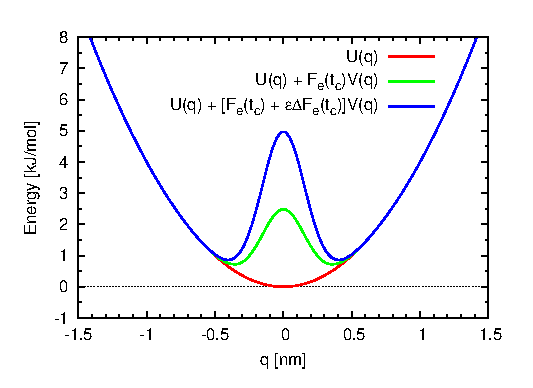
\includegraphics[width=0.4\textwidth]{figs/fig-split-pot.eps}
  \caption{The single-well potential with  splitting driving
    force. Time $T = 20$ ps.  Since the driving force is
    of gradient form, $ D( q) = -\nabla_{q}V( q)$,
    we plot the nonequilibrium driving energy of the system.  The red,
    green and blue lines are the potential energy without
    nonequilibrium driving, with nonequilibrium driving and
    the nonequilibrium driving perturbed by $\eps\delta u(t)$,
    respectively.  }
  \label{fig:tmp4}
\end{figure}

We use the idea of nonequilibrium linear response to investigate the
nonequilibrium phase space probability density distribution, denoted by $\rho^\eps(q, p, t)$, of a one-dimensional model system: one particle in a
splitting single-well potential as shown in Fig.~\ref{fig:tmp4}.  For convenience, we let the mass of
the particle to be 1~\textsf{amu}, and the friction coefficient to be
$1\,\textsf{ps}^{-1}$.
The temperature is the
room temperature $300\ \textsf{K}$, $k_BT = 2.48$~\textsf{kJ/mol}.
The unperturbed Hamiltonian of the system is
given by:
\begin{align}
  H ( p,  q) = \frac 12  p^2 + U( q) 
\end{align}
with potential
\begin{align}
  U( q) = \frac12\,k\, q^2 
\end{align}
Here $k = 8$~$\textsf{kJ} / (\textsf{mol nm}^2)$.
See the red line in Fig.~\ref{fig:tmp4} for the  potential $U$.
%$\textsf{kJ} / (\textsf{mol nm}^4)}$
The nonequilibrium driving $ D$ is given by a force of gradient form:
\begin{align}
   D( q) = -\nabla_{ q} V( q) ,
\end{align}
where the driving potential $V( q)$ has a Gaussian profile:
\begin{align}
  V( q) = \frac{1}{\sqrt{2\pi \sigma^2}}
  \exp\Big\{-\frac{ q^2}{2\sigma^2}\Big\}
\end{align}
we use $\sigma = 0.16$~\textsf{nm}.  The strength of nonequilibrium
driving $u(t)$ is set to be linearly growing, i.e. $ u(t) = k_e\cdot t/T$,
where $k_e$ is a unitless constant.
We
consider the perturbation to the system given by $\eps\delta u(t) = \eps k_e \cdot t/T$.
We consider the following parameters: end time $T = 20$~\textsf{ps}, 
$k_e = 1$ and $\eps = 1$, see Fig.~\ref{fig:tmp4}
for the nonequilibrium driving potential and perturbed
potential at time $t = T$. The initial distribution $\rho^0(q, p, 0)$ is set to
be equilibrium distribution of the unperturbed system.
\recheck{
  We use Euler scheme with time step of $10^{-4}$ to discretize the
  Langevin equation. The inital configurations for nonequilibrium
  simulation are generated by taking configurations
  from an equilibrium simulation of $10^6$~\textsf{ps} at an 1~\textsf{ps} time interval.
  Then starting with these inital configurations,  the nonequilibrium
  Langevin equation is integrated until 20~\textsf{ps} with the same numerical
  scheme and time step.
}

\begin{figure}
  \centering
  \includegraphics[width=0.95\textwidth]
  {figs/fig-split-str2-2d-distrib-no2nd.eps}
  \caption{ The plot of $ \rho^\eps(q,p,t)$ in  phase
    space under the perturbed nonequilibrium driving described in the text. From left to right the columns present results at times $t =
    0$, 5, 10 and 20~\textsf{ps}.  First row: Results of a brute force
    nonequilibrium simulation. Second row: Results of
    classical equilibrium linear response theory, see the text for details. Third row: Results using the
    nonequilibrium linear response result.  }
  \label{fig:tmp6}
\end{figure}

Fig.~\ref{fig:tmp6} presents the numerical results for  the phase space probability distribution for the splitting
single-well potential. From left to right the four columns present the
distribution of the system at time $t = 0$, 5, 10 and 20~\textsf{ps}. The first
row presents the result of a brute force nonequilibrium simulation.  It is clear
that at the beginning the distribution has only one peak around $q = 0$ and $p = 0$. As  time evolves, an energy barrier develops
in the center of the simulation region and, therefore, the single peak
splits into two equally sized peaks.  In the end, the two
peaks are entirely seperated.  The brute force nonequilibrium
simulation serves as the precise result to which the response theory
should be compared. The second row shows the result of the
traditional equilibrium linear response theory.  Please notice that in
this case, since the reference simulation is in equilibrium, we set the perturbation to
\[
\eps v_t = D(q) (u_t+\eps\delta u_t)=2\eps D(q)k_e\cdot t/T=2\eps D(q)\delta u_t,
\] 
so that the effective perturbation is of strength $2\eps = 2$.  At $t \leq
15$~\textsf{ps}, the accuracy of the equilibrium linear response is
perfect. At $t =
20$~\textsf{ps}, magnitude of the peaks are relatively too strong,
and in the gap between them the distribution is actually negative.
Since the probability distribution is always positive, the
numerical solution of the equilibrium linear response is qualitatively wrong.
The poor accuracy is due to the fact that the strength of perturbation is no
longer small so that the preliminary assumption of the classical reponse theory ("small perturbation")
is not satisfied.  

The third row of Fig.~\ref{fig:tmp6} presents the results computed using the novel nonequilibrium  linear response formula: we first start form the equilibrium distribution, apply  $u(t)$, arrive at a nonequilibrium distribution and then, in a second step, compute the effect of the nonequilibrium driving $\delta u(t)$.  The numerical results are satisfactorily consistent with
the brute force nonequilibrium simulation, because the perturbation is still  small enough and the novel linear response theory achieves
good accuracy.

% Fig.~\ref{fig:tmp6} presents the numerical results of perturbation $\eps =
% 2$.  Only with a linear response calculated from the equilibrium
% simulation (2nd row), the stability of the two new core sets are too
% strong, and the unstable region between them is over estimated, comparing with
% the brute force simulation presented on the first row.
% We present the  second order response results on the 3rd row, which is
% also calculated from the equilibrium simulation. In this case, the statistical
% error is too large, so that
% the profile of $\mt_\tau f$ is indeed too noisy to draw any useful information.
















% \subsection{The tilting double-well potential}


% We test the idea firstly by a one-dimensional model system: one particle in a
% tilting double-well potential. For convenience, we let the mass of the
% particle to be 1~\textsf{amu},
% and the friction coefficient to be $1\,\textsf{ps}^{-1}$.
% The unperturbed
% Hamiltonian of the system is given by:
% \begin{align}
%   \mh ( p,  q) = \frac 12  p^2 + U( q) 
% \end{align}
% with potential
% \begin{align}
%   U( q) = \frac12 k ( q^2 - a^2)^2
% \end{align}
% Here $k = 8$~$\textsf{kJ} / (\textsf{mol nm}^4)$, and $ a = 1\ \textsf{nm}$.
% At room temperature $300\ \textsf{K}$, $k_BT = 2.48$~\textsf{kJ/mol}.
% The red line in Fig.~\ref{fig:tmp1} presents the unperturbed potential.
% %$\textsf{kJ} / (\textsf{mol nm}^4)}$
% The perturbation is given by
% \begin{align}
%    D( q) = -\nabla_{ q} V( q) = 1
% \end{align}
% Here $V( q) = - q$   effectively tilts the original
% potential $U( q)$ (see the gree and blue lines in Fig.~\ref{fig:tmp1}).
% The strength of $u(t)$ is
% set to be $k_e$, when the time $t$ is larger than some warm-up time $t_c$.
% When $t \leq t_c$, the strength of $u(t)$ is linearly growing,
% i.e. $ u(t) = k_e\cdot t/t_c$.
% We use the value $t_c = 20$~\textsf{ps}, so that the perturbation increases slow
% enough: the typical decaying time scale of the correlation function
% in~\eqref{eqn:eq-lr} is roughly 3~\textsf{ps}.
% We choose $\tau = 1$~\textsf{ps}, and
% % We choose $\mt_\alpha$
% % to be the propagator of the Langevin dynamics at temperature $150$
% % \textsf{K} with $\alpha = 1$ \textsf{ps}.
% consider the stability of the
% distribution $f( x, t)$ at time $t$: $\Delta\mt_\tau f( x, t)$.
% The larger
% this value, the more stable the core sets are.

% See Fig.~\ref{fig:tmp2} and \ref{fig:tmp3} for numerical result.  Both
% the results of the brute-force nonequilibrium simulation
% and that of the response theory are presented.
% In Fig.~\ref{fig:tmp2},
% the good agreement between the brute-force (1st row)
% and the linear response result (2nd row) indicates that $\eps = 2$ is
% indeed a relatively small perturbation to the equilibrium.
% In the third row of Fig.~\ref{fig:tmp2},
% the second order response is considered. We do not see any
% substantial improvement of the result by including this higher order term,
% because the
% driving force to the system is small,
% and the linear term is anyway a good approximation.

% In Fig.~\ref{fig:tmp3}, as the
% perturbation grows stronger, the left well becomes less stable, while
% the right well becomes more stable.  When the perturbation is as strong as
% $\eps = 4$, the linear response result (2nd row) is no
% longer precise:
% At $t\geq 20$ \textsf{ps}, the left well basically
% disappears, however, the linear response calculation presents
% artificial structure (that is a small artificial
% stable region accompanied by a small unstable region)
% at the position of the left well.
% The second order response (3rd row) improves the accuracy a little, 
% however, it also includes artificial finer-grained oscillation in the profile.
% At the same time, the numerical uncertainty is higher, so the figure
% looks noisy.
% In the 4th row of Fig.~\ref{fig:tmp3}, we present the linear response result
% that calculate from 
% a intermediate
% nonequilibrium simulation with driving force of $k_e = 2$.
% Notice that the reference simulation in this case is also a
% nonequilibrium simulation, so the effective strength of perturbation
% is reduced to $\eps = 2$. According to Fig.~\ref{fig:tmp1}, this can be
% considered as a small perturbation.
% A substantial improvement is achieved: the profile
% is correctly calculated, and the statistical error is small.

% % the 1st order result of the
% % response formula~\eqref{eqn:pert-approx-1} and
% % \eqref{eqn:pert-approx-2}, with
% % respect to the reference state $F_e^{\textrm{max}} = 2$. The result
% % is impressively improved compared with the linear response with respect to the
% % equilibrium state.


\subsection{Optimal tilting of a double-well potential}
\begin{figure}
  \centering
  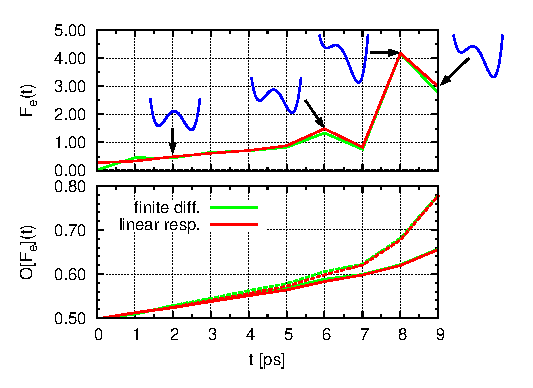
\includegraphics[]{figs/fig-ctr-stat-2.eps}
  \caption{Illustration of the optimal control for tilting the potential.  
    In this plot, $T=9$ ps.  Top panel: Optimal control $o_t$ as calculated based on a family of piecewise linear ansatz functions with time interval 1~ps; the blue insertions show the shape of the nonequilibrium driving potential $U + o_t V$ at the times indicated by the black arrows. Bottom panel: Optimal gain $I=F(o_t)$ (solid lines) and the probability $P$ of being in the right well associated with $o_t$ (dashed lines) as functions of time along the optimal control. Red lines: computation using   the nonequilibrium linear response theory. Green lines: brute force computation as described in the text. }\label{fig:tmp7}
\end{figure}

In this section, we consider the following double well potential:
\begin{align}
  U( q) = \frac12 k ( q^2 - a^2)^2
\end{align}
Here $k = 8$~$\textsf{kJ} / (\textsf{mol nm}^4)$, and $ a = 1\
\textsf{nm}$.  See the leftmost blue insertion of Fig.~\ref{fig:tmp7} for
the shape of the potential.
%$\textsf{kJ} / (\textsf{mol nm}^4)}$
The perturbation is given by a gradient form tilting of $U( q)$ by means of
\begin{align}
   D( q) = -\nabla_{ q} V( q) = 1,
\end{align}
with $V( q) = - q$. We want to
optimally design the tilting such that the probability
of being in the right well is as high as possible 
at the end time of the process under a constraint on the energy used for the control in the sense of
the following optimal forcing problem:
\begin{align}
  \tilde{I} & = \max_{u_t \in\mathcal F} \bE_{\rho^0}\left[ -\int_{0}^{T} \frac{1}{2}|u_{s}|^{2}\,dt + L(q_T) \right],
\end{align}
with $L(q_T)=\chi_{[a-\delta,a+\delta]}(q_T)/\eta$ representing the probability of the end point of the trajectory, $ q_T$, being in the right well ($\chi_I$ denotes the indicator function of the interval $I$) with $\eta$ being a weighting constant, ${\mathcal F}$ denoting the space of function that are piecewise linear  on $[0, T]$ in uniform intervals of length 1 ps, and $\rho^0$ being the
\recheck{initial nonequilibrium distribution $\rightarrow$ nonequilibrium distribution under control $u_t$}. With $P(T) = \eta \bE_{\rho^0}(L(q_T))$, the probability of ending up in the right well at time $T$, and $I=\eta \tilde{I}$ we thus have
\[
  I = \max_{u \in\mathcal F} F(u),\quad F(u)= P(T) -
  \frac{\eta}{2}\,
   \int_0^T |u_t|^2\, dt\,.
   \]
   \recheck{shall we use $I(u)$ instead of $F(u)$?, so that the
     notation is consistent with  Sec. 3.}
 It is
clear that for an unbiased double-well, $P(T)$
is 0.5 if we choose $\rho^0=\rho_0$ as initial distribution.  The integral is the ``cost'' of the control and $\eta$  indicates the relative magnitude of the
cost. 

\recheck{ In all our numerical tests for the optimal control problem, the
  Langevin dyanmics Eq.~\eqref{ocp1} is discretized by the Euler
  scheme with a time step of $10^{-3}$~\textsf{ps}.
  The initial distribution $\rho^0(q,p,0)$ is also set to be the
  equilibrium distribution $\rho_0$ of the unperturbed system.
  Therefore, an equilibrium simulation of $10^6$~\textsf{ps} is firstly performed (with
  the same numerical scheme and time step), and
  configurations are saved every 10~\textsf{ps} (in total $10^5$
  configurations) along the trajectory.
  Then by using these configurations as inital configurations,
  $10^5$ nonequilibrium
  trajectories are integrated until 9~\textsf{ps}, while at the same time
  the nonequilibrium responses are calculated and then averaged to
  estimate the ensemble average on the r.h.s of Eq.~\eqref{dida}.
  The statistical
  uncertainty of this estimate varies by each step of iteration, but
  is roughly $7\times10^{-4}$.  The statistical uncertainty for the 
  optimization target $I$ is roughly $1\times10^{-3}$.
  % The gradient search~\eqref{gd} is performed with a constant increment
  % $\tau_n = 30$.
}

Fig.~\ref{fig:tmp7} presents the numerical results of $\eta = 0.01$.
Starting from an initial guess of linear control from $u_0 = 0$ to
$u_T = 1$,
the gradient search~\eqref{gd} \recheck{uses a constant $\tau_n = 30$ and} converges at the 22nd step, when the
maximum increment of the control coefficient $\max_k\vert \delta a_k\vert$
is smaller than $0.02$, the termination threshold.
The magnitude of the optimal
control 
\[
o_t = \textrm{argmax}_{u_t \in\mathcal F} F(u_t)
\] 
is presented in the upper panel of Fig.~\ref{fig:tmp7},
with blue insertions showing the shape of the time-dependent optimal control potential 
$U(q) + o_t V(q)$ (optimally tilted double-well potential). 
The maximum $I$ and the corresponding optimal probability to end up in the right well are
given as functions of time in the lower plot by the solid and dashed lines, respectively.
The red lines in the figure are produced by the nonequilibrium
linear response theory developed in this work, i.e., using~\eqref{dida},
and the green lines represent the brute force reference simulations that has been performed as follows: The optimal control from ${\mathcal F}$ is calculated by a gradient descent based optimization method in which the gradient of the functional with respect to the control is computed by numerical differentiation (central finite differences) in each step.
% : \redc{$\partial I / \partial a_k \approx (I^+ - I^-) / (a_k^+ - a_k^-)$}
The good agreement between the red and green lines demonstrates that 
the linear response theory computes the gradient correctly.
Please note that in order to calculate the gradient by the finite difference scheme, one
needs to do $2K$ nonequilibrium simulations
(where $K$ is the dimension of ${\mathcal F}$; here $K = 10$). In contrast, the nonequilibrium response theory only needs one nonequilibrium simulation.


When $t<8$~\textsf{ps}, the magnitude of the control is still small.  Near the end time $T$, the magnitude of the control firstly
quickly goes up, and then falls down a little bit.  This implies some
interesting information.  If the system were able to immediately relax
to its equilibrium state (sometimes called
quasi-equilibrium), the population in the right well (dashed lines in
Fig.~\ref{fig:tmp7}) would immediately go down, as the control
decreases.  The fact that this does not happen, indicates that the
speed of changing the control is relatively fast compared to the 
time scale of quasi-equilibration of the system, so the system does not have enough time to
fully relax. Therefore, the observed phenomenon is truly
nonequilibrium, and our nonequilibrium linear response theory is a
tool that facilitates the investigation of this optimal forcing
problem in the nonequilibrium setting. The fact that the optimal control is decreasing at the end of the interval is understandable since the population in the right well needs time to be build and increasing the control till the very end would be a waste of energy without corresponding gain in population.

 
% Intuitively, one concludes
%that as the control goes up, the population in the right well actually
%does not have enough time to go as high as it could be, so when the
%control decreases, it continues going up rather than following the
%decreasing control.





\section{Conclusions and Remarks}

We derived  first and second order response formulas for molecular dynamics (driven Langevin dynamics) starting from general nonequilibrium distributions. For the special case of the initial distribution being the equilibrium distribution of the unperturbed dynamics, the novel linear response formula simplifies to the well-known standard formula. We validated the  formula in numerical experiments in comparison to brute-force nonequilibrium simulations. There, we demonstrated that the nonequilibrium linear response formula allows to extend the algorithmic use of linear response theory to significantly stronger perturbutions of the system since it permits intermediate steps based on partially propagated nonequilibrium distributions. 

By means of this theory we outlined how to use linear response theory for the computation of optimal controls in molecular dynamics where one desires to find the optimal perturbation/control that maximizes a target functional, that is, a certain expectation value (like the population of a certain region of state space) under a constraint on the energy used in the perturbation. Application of our nonequilibrium theory allows to compute the gradient of the target functional by computing expectation values \emph{only} for the dynamics at hand which permits efficient application of standard optimization techniques. We illustrated this technique in application to a simple test case and validated it in comparison to brute force optimization.  











\bibliography{ref}
\bibliographystyle{tMPH}





\end{document}